\documentclass[spanish, a4paper, 12pt, final, slideColor, nototal, colorBG, pdf, noaccumulate, darkblue] {beamer}
\usepackage[spanish]{babel}
\usepackage[utf8]{inputenc}
\usepackage{amsmath}
\usepackage{amssymb}
\usepackage{amsfonts}
\usepackage{latexsym}
\usepackage{mathtools}
\usepackage{anysize}
%\marginsize{2cm}{2cm}{2cm}{3cm}
\usepackage{soul}
\usepackage{mathtools}
\DeclarePairedDelimiter{\ceil}{\lceil}{\rceil}
\newcommand\eqdef{\stackrel{\mathclap{\mbox{\tiny{def}}}}{=}}
\newcommand\eqac{\stackrel{\mathclap{\mbox{*}}}{=}}

\usepackage{graphicx}
\usepackage{hyperref}
\usepackage{float}
\usepackage{verbatim}
\usepackage{caption}
\captionsetup{font=scriptsize,labelfont=scriptsize}
\DeclareGraphicsExtensions{.pdf,.png,.jpg}

\usepackage{import}
\usepackage{preamble}

\usetheme{Madrid}

\title{Estudio y desarrollo de técnicas para el testing de programas concurrentes}
\subtitle{CABS: traducción de C a ABS}
\author{Marco Antonio Garrido Rojo\thanks{\url{https://github.com/MaSteve/CABS-Slides}}}
\date{\today}

\begin{document}
\maketitle
\begin{frame}
  \frametitle{Introducción: historia y origen}
  \begin{itemize}
  \item En un principio, la mayoría de sistemas solo podían ejecutar una única secuencia de instrucciones a la vez.
  \item Con el avance de los ordenadores durante las últimas décadas del siglo pasado, se permite la ejecución simultánea de varios hilos de ejecución.
  \item Hoy en día es común el uso de la programación concurrente en la mayoría de aplicaciones y programas de todo ámbito.
  \end{itemize}
\end{frame}

\begin{frame}
  \frametitle{Introducción: inconvenientes}
  \begin{itemize}
  \item La ejecución paralela conlleva riesgos adicionales no presentes en los programas secuenciales.
  \item El principal problema que presenta es la presencia de una memoria compartida sobre la que los distintos hilos realizan modificaciones en cualquier momento.
  \item Asociado a esto, pueden ocurrir deadlocks, carreras de datos o comportamientos impredecibles.
  \end{itemize}
\end{frame}

\begin{frame}
  \frametitle{Introducción: soluciones}
  \begin{itemize}
  \item Podemos evitar que ocurran estableciendo restricciones mediante el uso de semáforos y cerrojos o implementaciones de algoritmos de más bajo nivel como el tie-breaker.
  \item El uso de estos mecanismos puede ser bastante \textbf{complejo}.
  \end{itemize}
\end{frame}

\begin{frame}
  \frametitle{Introducción: soluciones}
  \begin{figure}[h]
    \centering
    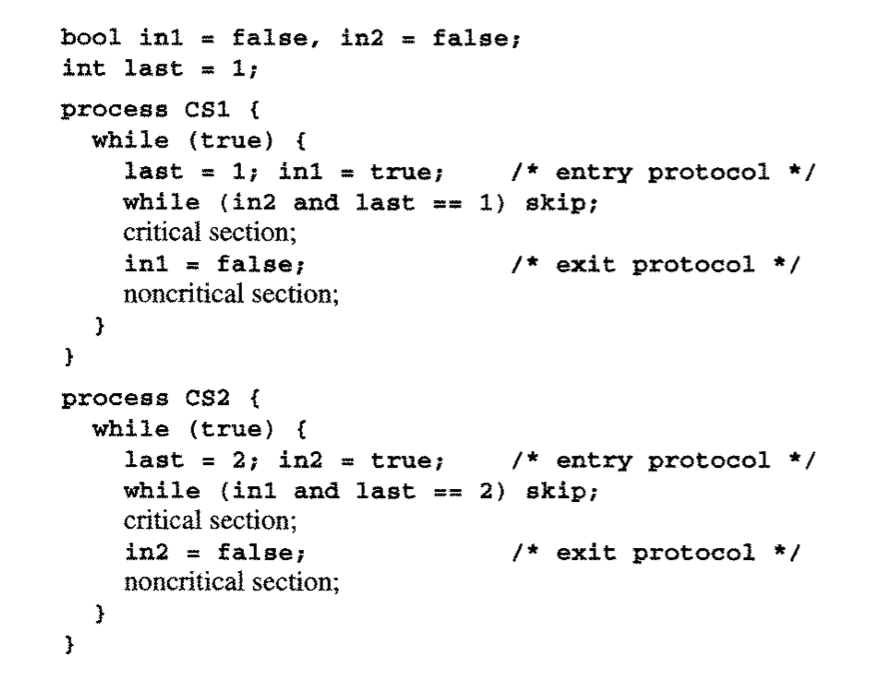
\includegraphics[scale=0.5]{tie-breaker.png}
    \caption{Algoritmo tie-breaker para dos procesos. (Andrews')}
  \end{figure}
\end{frame}

\begin{frame}
  \frametitle{Introducción: interleavings}
  \begin{itemize}
    \item En este terreno se sigue investigando para encontrar un modo definitivo que permita solucionar los problemas o detectarlos.
    \item Uno de los primeros asuntos estudiados es determinar el estado o estados finales a los que se llega ejecutando un programa concurrente.
  \end{itemize}
\end{frame}

\begin{frame}[fragile]
  \frametitle{Introducción: interleavings}
  \begin{lstlisting}
  int var;

  proc f1() {
    var := 1;
  }

  proc f2() {
    var := 2;
  }
  \end{lstlisting}
\end{frame}

\begin{frame}
  \frametitle{Introducción: interleavings}
  \begin{itemize}
  \item Explosión exponencial en el número de interleavings en proporción al número de hilos y al número de instrucciones.
  \item No siempre hay una correlación con el número de estados finales.
  \item No todos los interleavings tienen la misma importancia y algunos de ellos son equivalentes entre sí.
  \end{itemize}
\end{frame}

\begin{frame}[fragile]
  \frametitle{Introducción: interleavings}
  \begin{lstlisting}
  int var1;
  int var2;

  proc f1() {
    var1 := 1;  # 1
    var1 := 2;  # 2
  }

  proc f2() {
    var2 := 2;  # 3
    var2 := 1;  # 4
  }
  \end{lstlisting}
\end{frame}

\begin{frame}
  \frametitle{Introducción: grano}
  \begin{itemize}
  \item ¿Cuál es la atomicidad?
    \begin{itemize}
    \item Asignaciones atómicas: grano grueso.
    \item ¿Lectura de valores?: grano fino.
    \item ¡Secciones de código enteras!: \dots
    \end{itemize}
  \item ¿De qué depende el grano? ¿Qué ocurre si no hay memoria compartida?
  \end{itemize}
\end{frame}

\begin{frame}
  \frametitle{Introducción: actores}
  \begin{itemize}
  \item Cada objeto ejecuta sus tareas de forma concurrente con respecto a las del resto de objetos.
  \item Una única tarea a la vez por objeto. El resto de tareas esperan en una cola cuyo orden no es determinable.
  \item El paso de mensajes indica qué método desea ejecutar un objeto (pudiendo ser uno propio o perteneciente a otro objeto).
  \item Dependiendo del tipo de llamada, una tarea puede dejar paso a otra si aún no cuenta con los valores necesarios para proseguir.
  \item Se trata de una concurrencia donde el scheduler es non-preemptive.
  \end{itemize}
\end{frame}

\begin{frame}
  \frametitle{Introducción: ventajas}
  \begin{itemize}
  \item Reducción notable del número de interleavings: importante cuando se aplican técnicas de testing sistemático.
  \item Presente en lenguajes como Erlang, Scala y \textbf{ABS}.
  \item Cuenta con una amplia cantidad de herramientas, entre ellas, \textbf{SYCO}, que implementa \textbf{DPOR} para obtener los posibles resultados finales de un programa, reduciendo los interleavings redundantes.
  \end{itemize}
\end{frame}

\begin{frame}
  \frametitle{Introducción: objetivo}
  \begin{itemize}
  \item
  \end{itemize}
\end{frame}

\begin{frame} %%
  \frametitle{Introducción: soluciones}
  \begin{itemize}
    \item En este terreno se sigue investigando para encontrar un modo definitivo que permita solucionar los problemas o detectarlos.
    \item Cada vez es más necesario el uso de técnicas de validación como el testing.
    \item En esta línea es necesario detectar la redundancias de las distintas trazas de ejecución de un programa para crear tests más efectivos.
  \end{itemize}
\end{frame}

\begin{frame}
  \frametitle{ABS, SYCO y aPET}
  \begin{itemize}
    \item ABS es un lenguaje de modelado, orientado a objetos y concurrente que usa un modelo de paso de mensajes entre actores.
    \item Emplea llamadas asíncronas a objetos aislados unos de otros en términos de memoria.
    \item Cada objeto es capaz de gestionar un mensaje a la vez (e.g. reducción de la explosión de estados).
    \item Es posible usarlo con herramientas especializadas como SYCO y aPET para analizar implementaciones y generar tests para ellas.
  \end{itemize}
\end{frame}
\begin{frame}
  \frametitle{ABS y sus inconvenientes}
  \begin{itemize}
    \item Sintaxis compleja: interfaces y clases que las implementan, llamadas asíncronas\dots
    \item Boilerplate
    \item Alejado de las implementaciones reales (e.g. modelado e implementación separados).
  \end{itemize}
\end{frame}
\begin{frame}
  \frametitle{¿Qué es CABS?}
  La idea principal es tener un lenguaje de programación sencillo que
  \begin{itemize}
    \item Tenga una sintaxis similar a C.
    \item Permita ejecuciones concurrentes de grano fino de forma simple (mismo comportamiento que pthread).
    \item Tenga un tipado estricto y estático.
    \item Paradigma imperativo con funciones y arrays.
    \item Que pueda usar las mismas herramientas que ABS.
  \end{itemize}
\end{frame}
\end{document}
